\documentclass[tikz]{standalone}
\usepackage{fontspec}
\renewcommand*{\familydefault}{\sfdefault}
\usepackage{standalone}
%\usetikzlibrary{arrows.meta, decorations.pathreplacing, shapes.geometric}
\usetikzlibrary{bayesnet}

\begin{document}

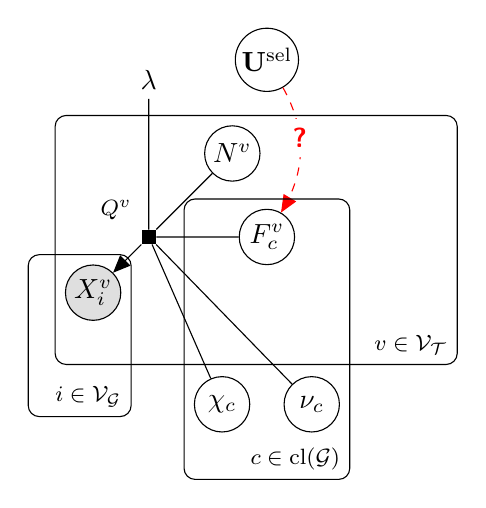
\begin{tikzpicture}

% Define nodes
\path (0,0)
node[obs] (X) {\(X^v_i\)}
%to
%(180:1.5 cm)
(X) +(0:4.5 cm) coordinate (tree)
(X) +(-0.7,-1) coordinate (site)
(X) +(45:1.0 cm) node[factor, label=above left:\(Q^v\)] (Q) {}
(Q) +(45:1.5 cm) node[latent] (N) {\(N^v\)}
(Q) +(0:1.5 cm) node[latent] (F) {\(F_c^v\)}
(Q) +(90:2.0 cm) node[] (bias) {}
%(Q) +(90:2.0 cm) node[] (mut) {\(\theta^\mathrm{mut}, \theta^\mathrm{co}\)}
(site -| F) coordinate (clique)
%(F) +(-0.7,-1.5) coordinate (clique)
(F) +(-75:2.2 cm) node[latent] (nu) {\(\nu_c\)}
(F) +(-105:2.2 cm) node[latent] (chi) {\(\chi_c\)}
(F) +(90:2.25 cm) node[latent] (U) {\(\mathbf{U}^\mathrm{sel}\)}
;

\node[fill=white, node font=\normalsize, align=center] (mut-cod) at (bias)
{\(\lambda\)}
;

\draw[->] (Q) -- (X);
\draw
(F) -- (Q)
(N) -- (Q)
(nu) -- (Q)
(chi) -- (Q)
(mut-cod) -- (Q)
;

\draw[dashed, red, ->] (U) to[bend left] node[font=\bfseries, pos=0.4, white, fill,
text=red] {?} (F);

% Plates
\plate {Xtree} {(X) (tree) (N) (F)} {\(v\in\mathcal{V}_\mathcal{T}\)} ;
\plate {Xsite} {(X) (site)} {\(i\in\mathcal{V}_\mathcal{G}\)} ;
\plate {Xclique} {(F) (nu) (chi) (clique)} {\(c\in\mathrm{cl}(\mathcal{G})\)} ;

\end{tikzpicture}

\end{document}


